\chapter{Dostępne rozwiązania}
\label{cha:dostepnerozwiazania}

Przed rozpoczęciem implementacji własnego rozwiązania postanowiono przeprowadzić badania mające na celu analizę aktualnie dostępnych rozwiązań spełniających przynajmniej w części założenia. Proces ten nie ma na celu znalezienie idealnego rozwiazania lecz poznanie różnych podejść do zagadnienia. Analiza różnych technologi które mogą być wykorzytane pozwoli na świadome wybranie najlepszych.


\section{Google Earth}
\label{sec:Google Earth}

Funkcjonalnośc interaktywnych map można znaleść w aplikacji stworzonej przez firmę Google. Program ten jest napisany przy użyciu języka C++, nie służy on do tworznia aplikacji mobilnych, dlatego nie został on wybrany jako kandydat do tworzonej pracy.

Aplikacja wykorzystuje statyczne obrazy będące zdjęciami satelitarnymi w przypadku obrazów z dużej wysokośći lub zdjęciami wykonanymi z pokładów samolotów. Pomimo duzej atrakcyjności ma ono bardzo ograniczoną możliwośći zmiany oglądanych danych, ograniczone do ilości wykonanych zdjęć, dodatkowo większość danych pochodzi z okresu ostatnich 60 lat.

Przykład takiej sytuacji został przedstawiony na rysunku \ref{fig:lasVegas1}, obraz terenu na którym powstanie miasto Las Vegas w roku 1950. Jak teren ten wyglądał w roku 1977 widzimy na rysunku \ref{fig:lasVegas2}, pomimo widocznych zmian teren ten nadal w dużym stopniu jest pustynny, dopiero na rysunku \ref{fig:lasVegas3} widzimy aktualny stan miasta.

Dzięki funkcji zmiany punktu i kąta patrzenia, pokazywania ciekawych miejsc czy chociażby włączania trybu w którym budynki nabierają formy przestrzennej, 3D, możemy poprzez zabawę i wirtualne wycieczki poszerzać naszą wiedzę o otaczającym nas świecie.


\begin{figure}[H]
  \centering
    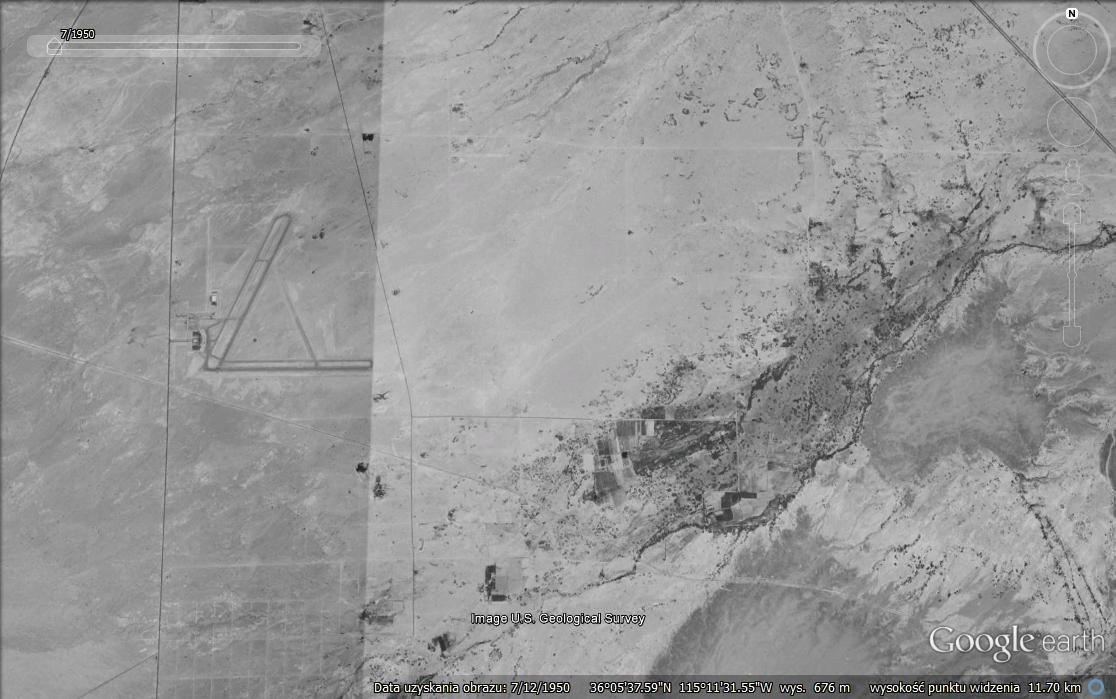
\includegraphics[width=100mm]{ge/01_1950.jpg}
  \caption{Las Vegas w 1950 roku.}
  \label{fig:lasVegas1}
\end{figure}

\begin{figure}[H]
  \centering
    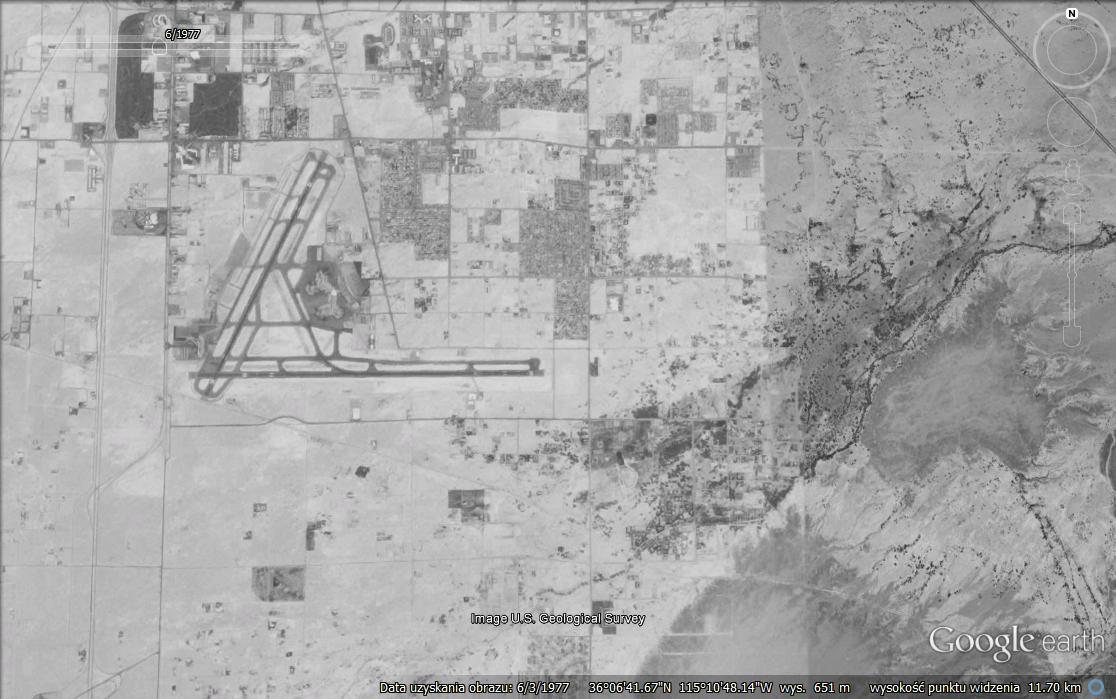
\includegraphics[width=100mm]{ge/02_1977.jpg}
  \caption{Las Vegas w 1977 roku.}
  \label{fig:lasVegas2}
\end{figure}

\begin{figure}[H]
  \centering
    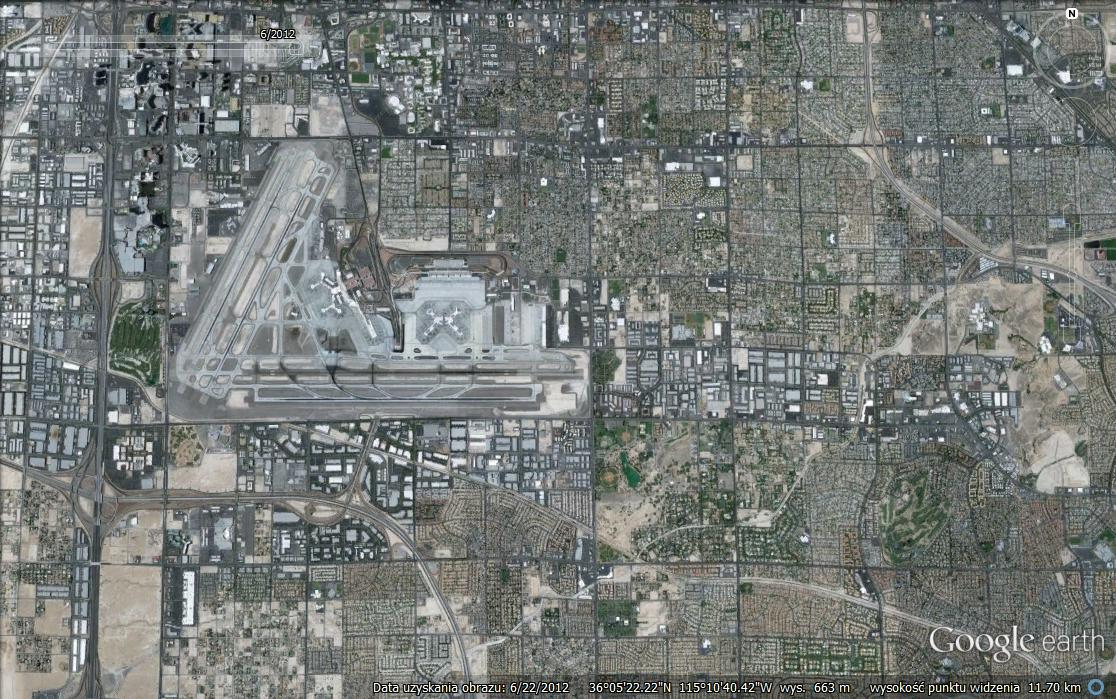
\includegraphics[width=100mm]{ge/03_2012.jpg}
  \caption{Las Vegas w 2012 roku.}
  \label{fig:lasVegas3}
\end{figure}

\section{Aplikacje wykonane w technologi Flash}
\label{sec:flashmap}

Podczas prac badawczych natrafiono na kilka aplikacji których główna część aplikcji została wykonana w technologi flash. Przykładami są interaktywna mapa historii europy \cite{worldology} czy mapa prezentująca zmianę granic państw w XX wieku \cite{flashborder} przykład na rysunku \ref{fig:flasheurope}. Oba projekty zawierają bogatą szatę graficzną, ich wykonanie jest bardzo estetyczne.
Zaletą tworzenia programów w tej technologi jest wykorzystanie mocy obliczeniowj karty graficznej do wyświetlania obrazów(dostępne od wersji 10.1 \cite{flashfrapghic}), dzięki temu procesor jest może wykonywać inne zadania.

\begin{figure}[H]
  \centering
    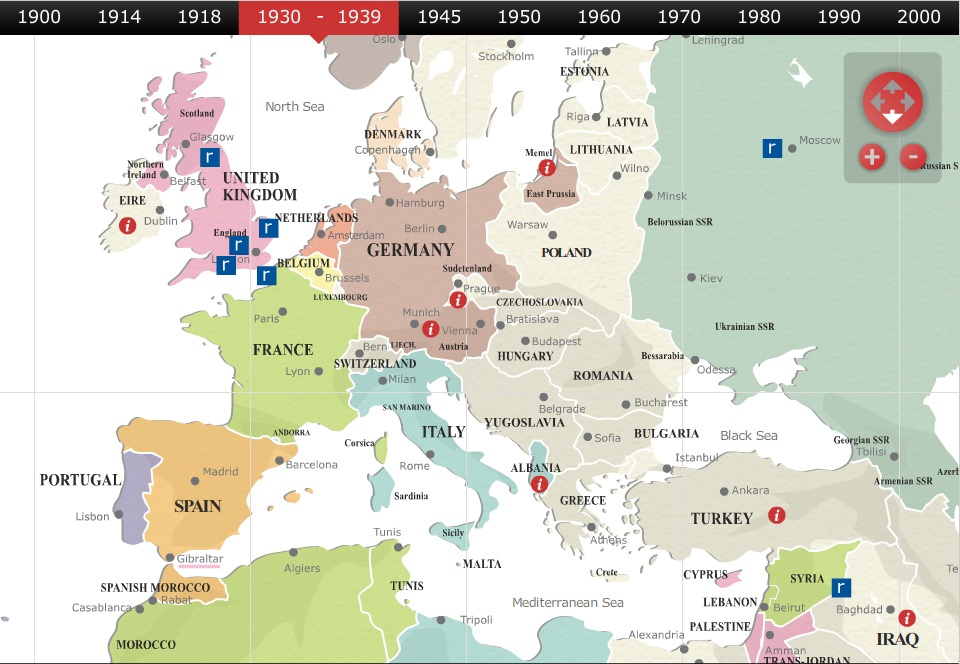
\includegraphics[width=130mm]{ge/archives.jpg}
  \caption{Europa w latach 30.}
  \label{fig:flasheurope}
\end{figure}


Wykorzystanie języka ActionScript wydaje się dobrym wyborem, niestety posiada kilka wad które go eliminują. Pierwszą z nich jest brak wsparcia technicznego dla wszystkich urządzeń mobilnych, przez co jej wykorzystanie ogranicza rynek docelowy.
Wymagana jest instalacja detykowanego odtwarzacza który pozwala na korzystanie z programów stworzonych w tym języku.
Ponieważ tworzona aplikacja jest jednym komponentem wymagane jest całkowite ściągnięcie z serwera na lokalny komputer aby można było z niej korzystać. Ostatnim aspektem jest brak kompatybilności elementów flash-owych z głównymi wyszukiwarkami internetowymi, ich indeksacja jest utrudniona(możliwe jest jedynie wykorzystanie tagów) a ich zawartość całkowicie niewidoczna w procesie indeksowania. Z uwagi na powyższe wady technologia nie została wykorzystana w omawianej pracy.

\section{Wykorzystanie JavaScript}
\label{sec:pref}

Częśc aplikacji pracujących na danych geograficznych jest tworzona przy uzyciu skryptowego języka jakim jest JS. Przykład zastosowania jest widoczny w bibiotece ``amMap'' \cite{jsmapapp}. Pozwala ona na proste pisanie rozwiązań w których zapewniona interakcja z użytkownikiem podnosi wartość programu. Przykład mapy z osią czasu przedstawiony na rysunku \ref{fig:jsheatmap} wskazuje rozkład średniej rocznej temepratury w stanach ameryki północnej na w przeciągu ostatnich 50 lat.

\begin{figure}[H]
  \centering
    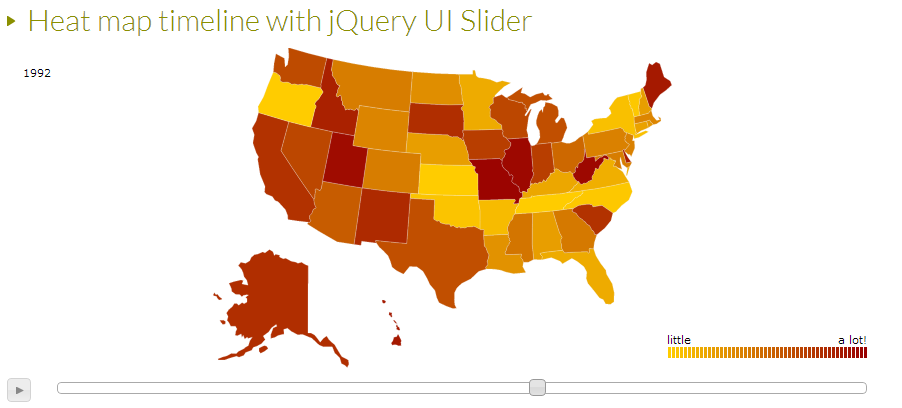
\includegraphics[width=130mm]{ge/jsheatmap.png}
  \caption{Mapa ciepla w USA.}
  \label{fig:jsheatmap}
\end{figure}

\section{Wybrane technologie}
\label{sec:technologie}

Po analizie dostęnych rozwiązań zdecydowano się na wykorzystanie w pracy następujących technologi.
\begin{itemize}

\item
HTML 5 - język HTML jest budulcem każdej strony internetowej, w wersji piątej zostały dodane rozwiązania które zwiększają jego możliwości

\item
JavaScript - umożliwia interakcję użytkownika ze stroną internetową  i zmiany konkentu bez konieczności odświeżania całej zawartości

\item
Less - agrgeguje i porządkuje style CSS

\end{itemize}
